\documentclass{article}

\usepackage[utf8]{inputenc}
\usepackage{graphicx}
\usepackage{tikz}
\usepackage{float}
\usepackage{wrapfig,lipsum}
\usepackage{svg}
\usepackage{mathtools}
\usepackage{tabu}
%\usepackage{subcaption}
\usepackage{subfigure}
\usepackage[a4paper, total={6in, 8in}]{geometry}

\begin{document}


\newcommand{\vecthreeBF}[1]{\vec{\textbf{#1}}}
\newcommand{\vecthree}[1]{\vec{#1}}

\newcommand{\parDeriv}[2]{\frac{\partial #1}{\partial #2}}
\newcommand{\parDerivS}[2]{\frac{\partial^2 #1}{\partial #2^2}}
\newcommand{\derivS}[2]{\frac{d^2 #1}{d#2^2}}

\newcommand{\dotProdBF}[2]{\vecthreeBF{#1} \cdot \vecthreeBF{#2}}
\newcommand{\dotProd}[2]{\vecthree{#1} \cdot \vecthree{#2}}

\newcommand{\crossProdBF}[2]{\vecthreeBF{#1} \times \vecthreeBF{#2}}
\newcommand{\crossProd}[2]{\vecthree{#1} \times \vecthree{#2}}


\newcommand{\fromeq}[1]{\textit{equation \ref{eq:#1}}}
\newcommand{\fromeqs}[2]{\textit{equations \ref{eq:#1} and \ref{eq:#2}}}

\newcommand{\fromfig}[1]{\textit{figure \ref{fig:#1}}}
\newcommand{\fromfigf}[4]{\textit{figures \ref{fig:#1}, \ref{fig:#2}, \ref{fig:#3} and \ref{fig:#4}}}

\newcommand{\fromsec}[1]{\textit{section \ref{sec:#1}}}

%----../../..++++.

%%%%%%

\section{Particle Accelerators}

Particle accelerators are sophisticated scientific instruments designed to accelerate charged particles, such as electrons, protons, or ions, to high speeds and energies. 
These accelerators play a crucial role in advancing our understanding of the fundamental properties of matter and the universe. 
They are widely used in various fields of research, including particle physics, nuclear physics, materials science, and medicine.

At their core, particle accelerators utilize electromagnetic fields to impart energy to particles and control their trajectories. 
These fields are generated by intricate arrangements of electromagnets and RF (radiofrequency) cavities within the accelerator structure. 
By precisely controlling these fields, accelerators can propel particles to speeds close to the speed of light, thus to high energies.

Accelerators can be categorized into two main types: linear accelerators (linacs) and circular accelerators. 
Linacs accelerate particles in a straight line, while circular accelerators use magnetic fields to bend the particle trajectory into a circular path. 

The acceleration process in accelerators involves multiple stages. Initially, particles are injected into the accelerator at a relatively low energy. 
As they progress through the accelerator, they are subjected to electric fields that accelerate them, while magnetic fields guide their trajectories.
Focusing elements, such as solenoid, dipole or quadrupole magnets, ensure the particles remain tightly controlled.

As particles gain energy in the accelerator, they approach relativistic speeds, where relativistic effects become significant. 
Special relativity governs the increase in mass and energy of the particles as they approach the speed of light, providing insights into the behavior of matter at high energies.
% TODO : ADD CIRCULAR AND LINEAR ACCELERATOR PICTURES HERE
\begin{figure}[H]
    \centering
    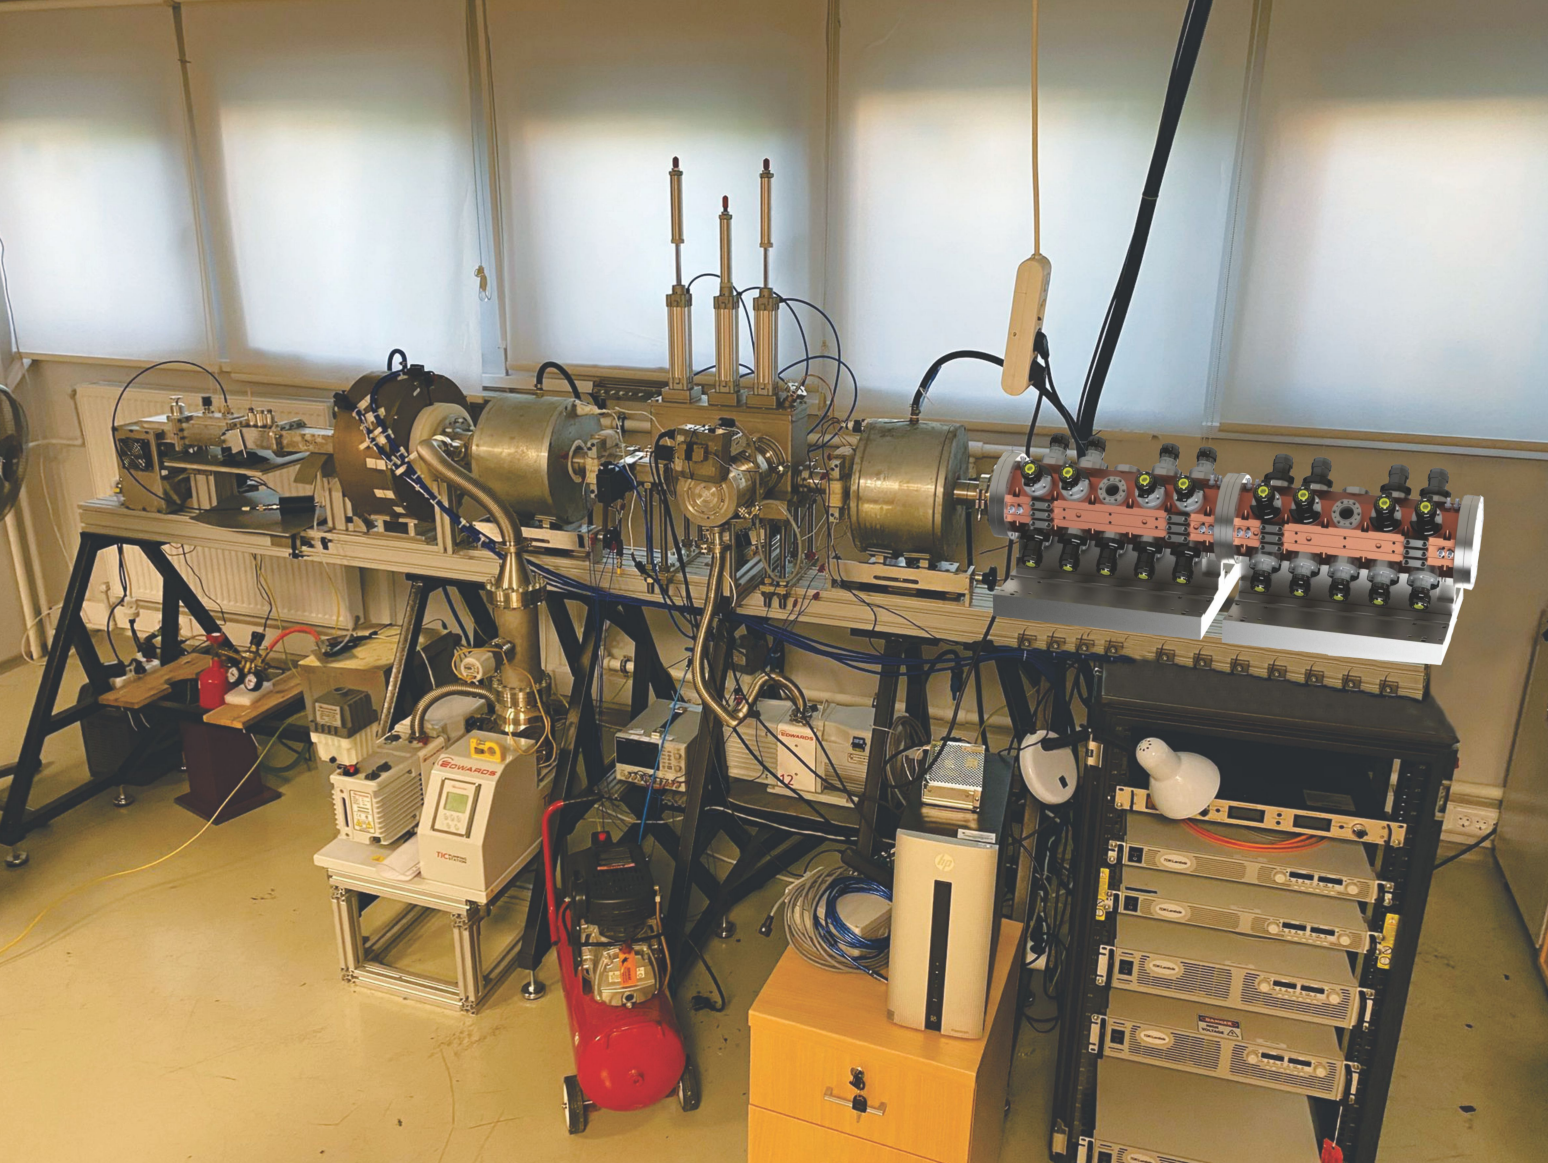
\includegraphics[width=.9\textwidth]{../../../figures/kahvelab_linac.png}
    \vspace{20pt}
    \caption{A linear proton accelerator in KAHVELab \cite{kahvelab_linac}.}
\end{figure}

\subsection{Acceleration Cavities} \label{sec:theory_cavities}
Radiofrequency (RF) cavities, also known as accelerating cavities or resonant cavities, are key components in particle accelerators. 
These cavities generate strong electromagnetic fields at specific frequencies to accelerate charged particles through clever engineering.

RF cavities are typically hollow metallic structures made of or coated with high-conductivity materials such as copper. 
The cavity is often cylindrical or spherical in shape, and its inner surface is polished to minimize energy losses through resistive heating.
The RF cavity is designed to be resonant, meaning that it naturally amplifies the electric fields at its resonant frequency. 
The resonant frequency is determined by the cavity's dimensions and the speed of light in the cavity material.

To achieve efficient energy transfer to the particles, the RF cavity is driven by an external RF power source operating at the resonant frequency. 
The power source supplies radiofrequency energy to the cavity, which causes the electric fields inside the cavity to oscillate at the desired frequency. 
These oscillating fields then transfer energy to the passing particles, increasing their kinetic energy by pushing and pulling on the charged particles as they pass through the cavity. 
\newline

\begin{figure}[H]
    \centering
    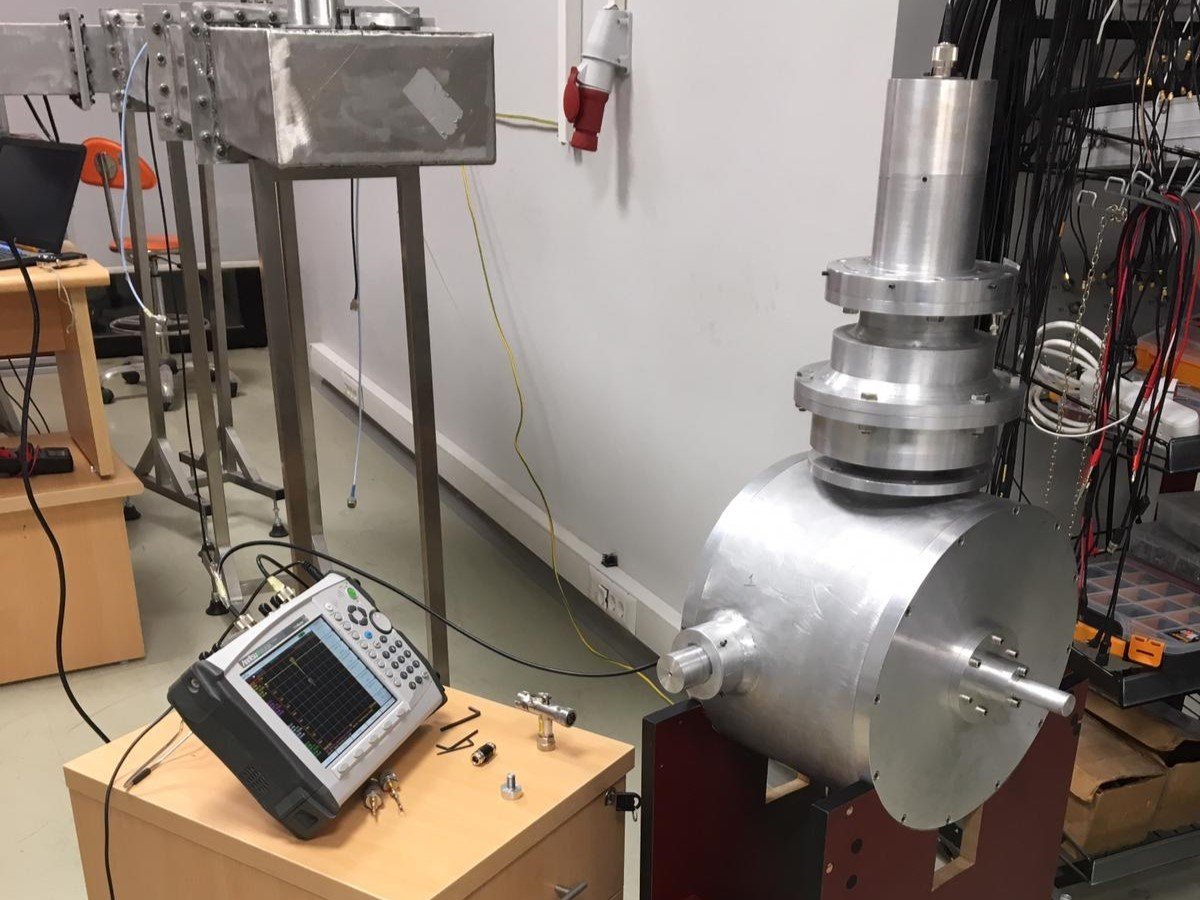
\includegraphics[width=.75\textwidth]{../../../figures/pill_box.jpeg}
    \vspace{20pt}
    \caption{An RF cavity used in KAHVELab.}
\end{figure}

In addition to accelerating the particles, RF cavities are often designed to provide focusing forces. 
By carefully shaping the cavity and adjusting the electromagnetic fields, the particles can experience focusing effects as they pass through the cavity. 
This helps to maintain a tight and controlled beam. To ensure efficient acceleration, it is essential to maintain phase stability. 
This means that the particles should experience the strongest electric fields at the correct time during their passage through the cavity. 
Precise timing and synchronization of the RF power source with the particle beam are crucial to achieve phase stability and maximize energy transfer.

\subsection{Bending Magnets}
Bending magnets, also known as dipole magnets, are fundamental components used in particle accelerators to control the trajectory of charged particles. 
They utilize the Ampere's Law to exert a magnetic field that interacts with the charged particles in the accelerator. 

According to the Lorentz Force Law (\fromsec{lorentz-force}), when a charged particle moves through a magnetic field, it experiences a force perpendicular to both its velocity 
vector and the magnetic field direction. This force causes the particle's trajectory to curve, resulting in a bending effect.


\subsection{Key Concepts}

\subsubsection{Resonance Frequency}
Resonance frequency is the frequency in which the electromagnetic fields form standing waves in a cavity.
It is determined by the physical dimensions and the speed of light in the cavity's medium. 
In a rectangular cavity for example, the resonance frequency can be calculated by
\vspace{-10pt}\begin{equation}
    f_{klm} = \frac{c}{2\pi \sqrt{\mu_r \epsilon_r}} \sqrt{(\frac{k}{w})^2 + (\frac{l}{u})^2 + (\frac{m}{v})^2}  ,
    \label{eq:f_r_rec}
\vspace{-10pt}\end{equation}
where $w$, $u$, $v$ are the dimensions of the cavity, $\mu_r$ and $\epsilon_r$ are relative permability and permittivity of the cavity respectably.

\subsubsection{Bunch}
Bunch refers to a tightly grouped collection of charged particles, such as electrons or protons, that are accelerated and maintained close together within a particle accelerator.

\subsubsection{Phase Stability}
Phase stability refers to the preservation of the timing relationship between particles and fields within an accelerator. 
It ensures that the phases of various electromagnetic fields or particles remain synchronized, 
which is crucial for achieving efficient particle acceleration. 
Maintaining phase stability is essential to prevent particles from becoming out of phase as they travel through accelerator structures, 
ensuring that they receive the correct energy boosts and interact predictably with detectors. 
Deviations in phase stability can lead to particle loss and decreased beam quality.

\subsubsection{Phase Lag}
Phase lag refers to the time delay between the oscillations of two interacting waveforms or particles. 
It describes the difference in phase angles within their respective cycles, between two signals. 

\subsubsection{Shunt Impedance}
The shunt impedance of an RF accelerator is a measure of the efficiency 
at which the accelerator can transform the supplied RF power into acceleration.
It is defined as
\vspace{-10pt}\begin{equation} \label{eq:shunt}
    Z_s = \frac{V_{acc}^2}{P_{diss}}  ,
\vspace{-10pt}\end{equation}
where $V_{acc}$ is the accelerating potential in which the particle is subjected to, 
$P_{diss}$ is the power dissipated on the cavity walls. 
An example \textit{shunt impedance} calculation can be found in \fromsec{cavity_of_a_rhodotron}.


\subsection{Rhodotron Accelerator} \label{sec:theory_rhodo}

Rhodotron Accelerator is a type of particle accelerator that was proposed by \textit{Jacques POTTIER} in 1989 \cite{rhodo_pottier}. 
First prototype was built at CEA Saclay later in 1992 \cite{rhodo_prototype}. It is named after the greek word for rose, \textit{rhodos}, due to the shape of the design \cite{rhodos}.

The design of a rhodotron mainly consists of a coaxial cylindrical RF cavity and bending magnets surrounding it. RF cavity is fed by an external RF source, accelerating the electrons entering from an attached electron injector.


\subsubsection{Acceleration cycle of Rhodotron}

Electrons undergo four different stages inside the accelerator. 
They are accelerated between the cylinderical plates and are shielded from the changing RF field while inside the inner cylinder and outside the cavity. 
This stages are explained further below.

%\begin{description}
%    \item[First acceleration] Electrons in the rhodotron cavity are accelerated by the electric field created between two coaxial cylinders, towards the inner cylinder when they are ejected into the cavity. (\fromfig{rhod_cycle_1})
%    \item[Inner shielding] While inside the inner cylinder, the cylinder acts as a faraday cage and shields the electrons inside while the electric field is being reversed. (\fromfig{rhod_cycle_2})
%    \item[Second acceleration] Once the electrons leave the inner cylinder, they accelerate towards the outer cylinder by the reversed electric field until they leave the cavity. (\fromfig{rhod_cycle_3})
%    \item[Recirculating Magnets] After leaving the cavity, an electromagnet placed in their path steers the electrons back into the cavity in which time the electric field changes the direction again. (\fromfig{rhod_cycle_4})
%\end{description}

\begin{itemize}
    \item \textit{First Acceleration:} Electrons in the rhodotron cavity are accelerated by the electric field created between two coaxial cylinders, towards the inner cylinder when they are ejected into the cavity (\fromfig{rhod_cycle_1}).
    \item \textit{Inner Shielding:} Inner shielding While inside the inner cylinder, the cylinder acts as a faraday cage and shields the electrons inside while the electric field is being reversed (\fromfig{rhod_cycle_2}). 
    \item \textit{Second Acceleration:} Once the electrons leave the inner cylinder, they accelerate towards the outer cylinder by the reversed electric field until they leave the cavity (\fromfig{rhod_cycle_3}). 
    \item \textit{Recirculating Magnets:} After leaving the cavity, an electromagnet placed in their path steers the electrons back into the cavity in which time the electric field changes the direction again (\fromfig{rhod_cycle_4}). 
\end{itemize}

This cycle can be repeated as long as real world constraints such as; placements and dimensions of the electromagnets, power requirements due to increasing magnetic field in order for sharper turns, can be overcomed.
After the desired amount of cycles, also called passes, has been completed, the electrons exit the accelerator.

This process is explained further in the \fromfigf{rhod_cycle_1}{rhod_cycle_2}{rhod_cycle_3}{rhod_cycle_4} where $T$ is the period of the electric field.

\subsubsection{Cavity of a Rhodotron} \label{sec:cavity_of_a_rhodotron}

Coaxial design of the cavity concentrates the electric field, while the magnetic field diminishes in the middle of the cylinders. 
Therefore the electrons are injected and accelerated in the plane of zero magnetic field where the electric field is strongest (\fromfig{rhodo_cavity_field_dist}).

\iffalse \begin{figure}[H]
    %\captionsetup[subfigure]{justification=centering}
    %\captionsetup{justification=centering}
    \centering
    \begin{subfigure}{0.45\textwidth}
        \centering
        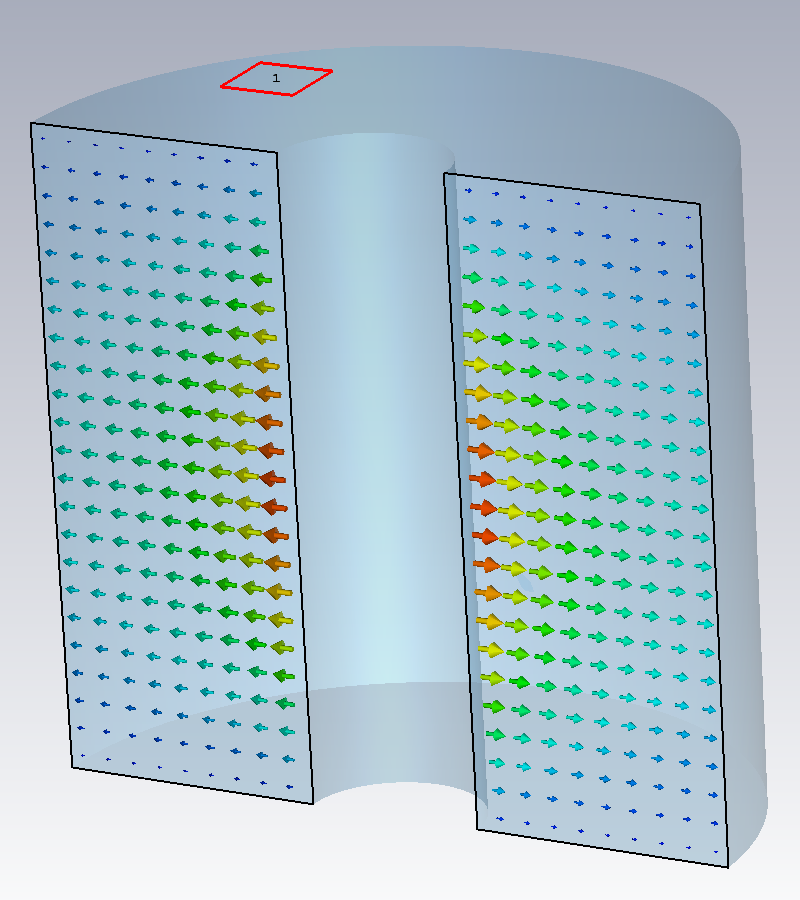
\includegraphics[width=\linewidth]{../../../figures/cst/cavity_E_field_dist.png}
        \caption*{$\vecthreeBF{E}$ field.}
    \end{subfigure}
    \begin{subfigure}{0.45\textwidth}
        \centering
        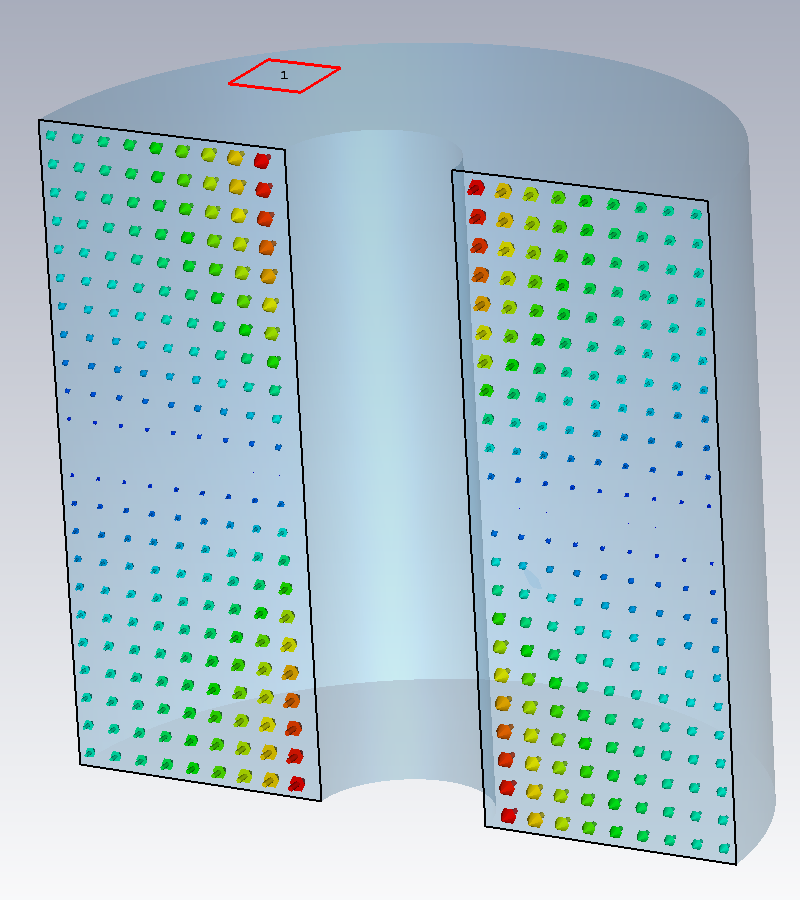
\includegraphics[width=\linewidth]{../../../figures/cst/cavity_B_field_dist.png}
        \caption*{$\vecthreeBF{B}$ field.}
    \end{subfigure}
    \caption{$\vecthreeBF{E}$ and $\vecthreeBF{B}$ eigenmode field distributions inside a coaxial cavity.}
    \label{fig:rhodo_cavity_field_dist}
\end{figure} \fi
\begin{figure}[H]
    \centering
    \subfigure[\centering $\vecthreeBF{E}$ field]{{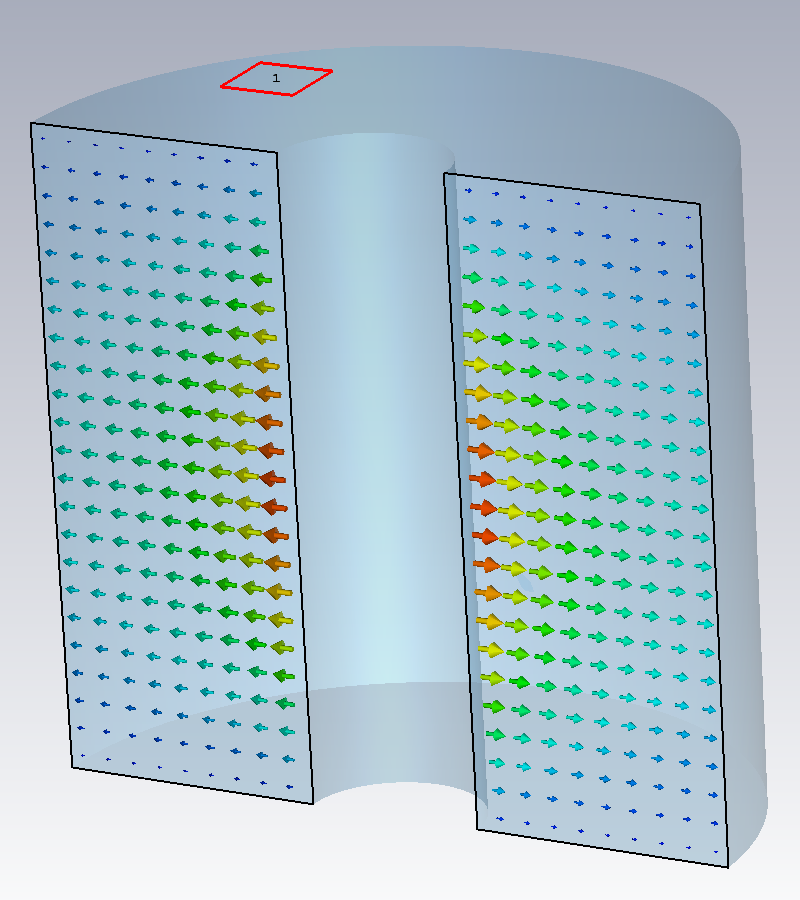
\includegraphics[width=0.45\textwidth]{../../../figures/cst/cavity_E_field_dist.png} }}%
    \qquad\subfigure[\centering $\vecthreeBF{B}$ field]{{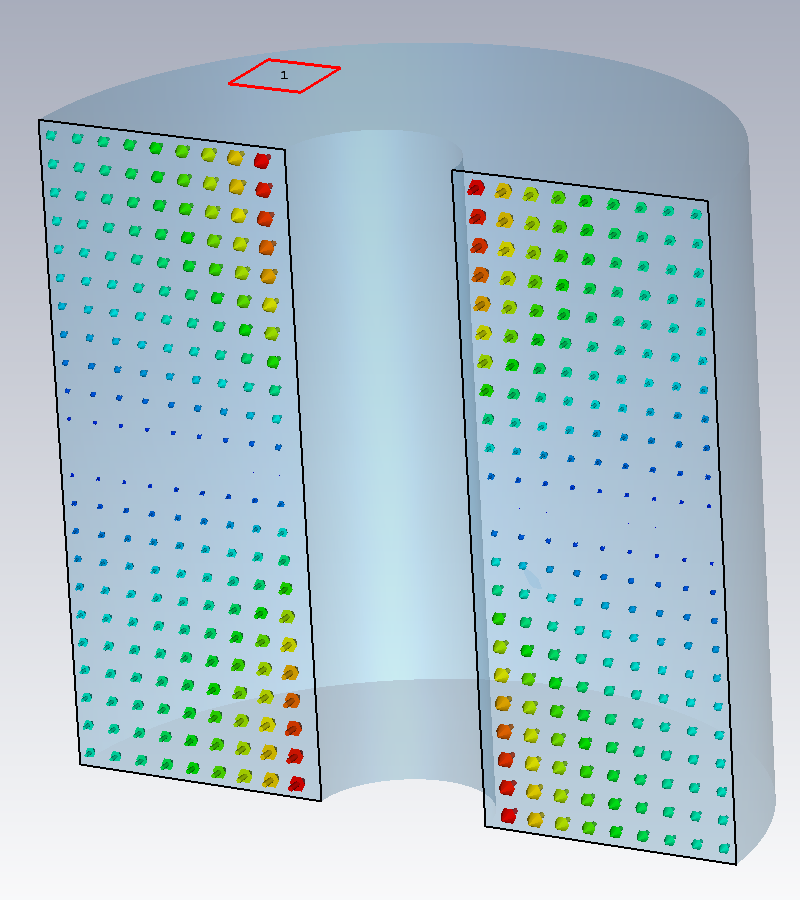
\includegraphics[width=0.45\textwidth]{../../../figures/cst/cavity_B_field_dist.png} }}%
    \vspace{20pt}
    \caption{$\vecthreeBF{E}$ and $\vecthreeBF{B}$ eigenmode field distributions inside a coaxial cavity.}
    \label{fig:rhodo_cavity_field_dist}
\end{figure}
For a cavity defined by the volume between two coaxial cylinders of equal lengths ($h$) with radii of $R_1$ and $R_2$, where $R_1 < R_2$, located at the origin (\fromfig{int_curve}),
first eigenmode solution of the $E$ and $B$ fields are \cite{rhodo_pottier}
\vspace{-10pt}\begin{eqnarray}
    E &=& \frac{E_0}{r} \cos\left( \frac{\pi z}{h} \right) \sin \left( \omega t + \phi \right)  , \\
    B &=& \frac{B_0}{r} \sin\left( \frac{\pi z}{h}\right) \cos\left( \omega t + \phi\right)  ,
\vspace{-10pt}\end{eqnarray}
where $\omega=2\pi f$, $f$ is the resonance frequency.

\begin{figure}[H]
    \centering
    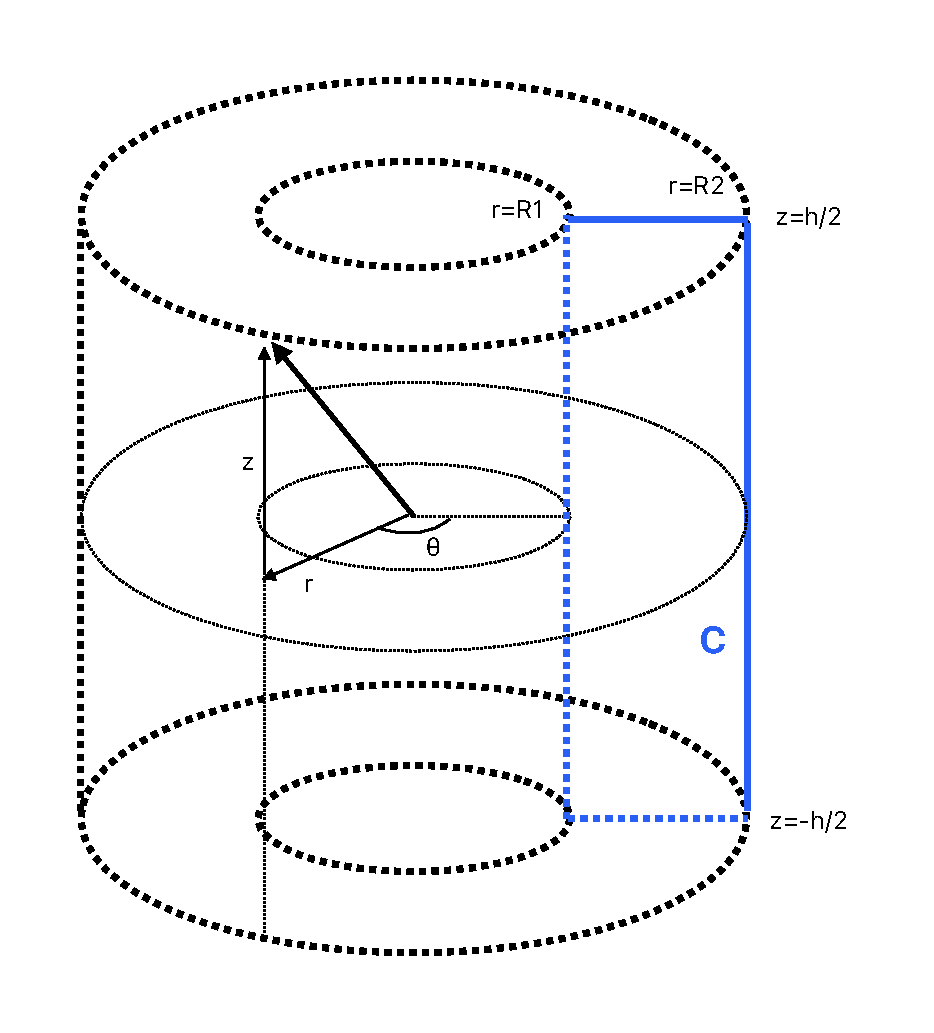
\includegraphics[width=.55\textwidth]{../../../figures/illustrations/rhodo_integral_curve.pdf}
    \vspace{20pt}
    \caption{Illustration of a simple coaxial cavity with the curve \textbf{C} in \fromeq{p_diss_C_curve}.}
    \label{fig:int_curve}
\end{figure}

Because acceleration potential is located on the $z=0$ plane and $\vecthreeBF{E} \parallel \hat{r}$, $V_{acc}$ can be found by
\vspace{-10pt}\begin{eqnarray} 
    V_{acc} &=& 2 \int_{R_1}^{R_2} |E|^2 dr \nonumber\\
            &=& 2 E_0 \int_{R_1}^{R_2} \frac{dr}{r} \nonumber\\
            &=& 2 E_0 \ln(\frac{R_2}{R_1}). \label{eq:v_acc}
\vspace{-10pt}\end{eqnarray}
Dissipated power $P_{diss}$, on the other hand, can be calculated as \cite{rf}
\vspace{-10pt}\begin{eqnarray} 
    P_{diss} &=& \frac{1}{2} \int \int \rho_s | H_{||} |^2 dA \nonumber \\
             &=& \frac{\rho_s}{2\mu_0^2} \int_0^{2\pi} \int_C | B_{||} |^2 r ds d\theta . \label{eq:p_diss_C_curve}
\vspace{-10pt}\end{eqnarray}
where $\rho_s$ is the areal skin resistivity ( $\rho_s \approx 2.51 \times 10^{-7} f^{1/2}$ for copper \cite{rhodo_pottier} ), $B=\mu H$, $\mu$ is permeability, $\mu_0$ is the vacuum permability. 
Integral curve \textbf{C} is defined as the circumference of cylindrically symmetrical cross sectional area of the cavity (\fromfig{int_curve}).
This curve can be seperated to its line components and total power dissipation of this curve, $P_C$ will be equal to sum of the power dissipated in these lines.
Since $\vecthreeBF{B}$ is always parallel to the surface we can use $\vecthreeBF{B}$ directly as
\vspace{-10pt}\begin{eqnarray}
    P_{diss} &=& \frac{\rho_s}{2\mu_0^2} \int_0^{2\pi} (
                   2\int_{0}^{\frac{h}{2}} |B|^2 r dz \Big|_{r=R_1}
                 + 2\int_{0}^{\frac{h}{2}} |B|^2 r dz \Big|_{r=R_2} 
                 + 2\int_{R_1}^{R_2} |B|^2 r dr \Big|_{z=\frac{h}{2}})d\theta \nonumber\\
             &=& \frac{\rho_s}{2\mu_0^2} \int_0^{2\pi} (2I_A + 2I_B + 2I_C)d\theta 
                 = \frac{2\rho_s \pi}{\mu_0^2}(I_A + I_B + I_C)   ,\\
    I_A &=& \int_{0}^{\frac{h}{2}} |B|^2 r dz \Big|_{r=R_1} = B_0^2 \frac{h}{4R_1}   ,\\
    I_B &=& \int_{0}^{\frac{h}{2}} |B|^2 r dz \Big|_{r=R_2} = B_0^2 \frac{h}{4R_2}   ,\\
    I_C &=& \int_{R_1}^{R_2} |B|^2 r dr \Big|_{z=\frac{h}{2}} = B_0^2 \ln(\frac{R_2}{R_1}) .
\vspace{-10pt}\end{eqnarray}
Inserting $H_0=B_0/\mu_0$, finally we have the dissipated power
\vspace{-10pt}\begin{equation} \label{eq:p_diss}
    P_{diss} = \rho_s \pi H_o ( \frac{h}{2R_1} + \frac{h}{2R_2} + 2\ln(\frac{R_2}{R_1}) ).
\vspace{-10pt}\end{equation}
Therefore, from \fromeq{shunt}, using \fromeqs{v_acc}{p_diss} also $E_0/H_0 = Z_0 \approx 120 \pi$ we have
\vspace{-10pt}\begin{eqnarray}
    Z_s &=& \frac{4E_0^2}{H_0^2 \pi \rho_s} \frac{ \ln^2(\frac{R_2}{R_1})}{(\frac{h}{2R_1} + \frac{h}{2R_2} + 2 \ln(\frac{R_2}{R_1}))} \nonumber\\
        &=& \frac{8 \pi 60^2}{\rho_s} \frac{ \ln^2(\frac{R_2}{R_1})}{(\frac{h}{4}(\frac{1}{R_1} + \frac{1}{R_2}) + \ln(\frac{R_2}{R_1}))}   ,
\vspace{-10pt}\end{eqnarray}
where, time dependencies have been removed from $\vecthreeBF{E}$ and $\vecthreeBF{B}$ 
and the maximum values for $V_{acc}$ and $P_{diss}$ have been used. 
However, particles do not interact with constant $\vecthreeBF{E}$ field during acceleration. 
Therefore, a more useful parameter called \textit{effective shunt impedance} can be defined as
\vspace{-10pt}\begin{equation}
    Z_{se} = Z_s T^2  ,
\vspace{-10pt}\end{equation}
where $T$ is the \textit{transit time factor}, a correctional coefficent that contain the changing field effects during acceleration.
\clearpage
For a relativistic electron crossing the axis at time 0, $T$ can be found by \cite{rhodo_pottier}
\vspace{-10pt}\begin{eqnarray}
    T &=& \frac{S_i(\frac{2 \pi R_2}{\lambda}) - S_i(\frac{2 \pi R_1}{\lambda})}{\ln(\frac{R_2}{R_1})}   ,\\
    S_i(\theta) &=& \int_0^{\theta} \frac{\sin(x)}{x} dx .
\vspace{-10pt}\end{eqnarray}

For a relativistic electron crossing the axis at $2\pi f t_0 = \phi$ on the other hand, $T$ needs to be multiplied by $\cos(\phi)$ as
\vspace{-10pt}\begin{equation}
    T(\phi) = T \cos(\phi) .
\vspace{-10pt}\end{equation} 
Putting all these calculations together, energy gain of a relativistic electron, passing the origin at $\phi / \omega$ as calculated by \textit{J. Pottier} is \cite{rhodo_pottier}
\vspace{-10pt}\begin{eqnarray}
    \Delta E &=& q V_{acc}^{ef} \nonumber\\
             &=& q Z_{se}^{1/2}P_{diss}^{1/2} \cos(\phi)  ,
\vspace{-20pt}\end{eqnarray}
where $ V_{acc}^{ef} = V_{acc} T(\phi)$ is the effective accelerating potential.
If $\Delta E$ is taken in \textit{MeV}, $Z_{se}$ in $M\Omega$ and $P_{diss}$ in \textit{MW}, this equality becomes
\vspace{-10pt}\begin{equation} \label{eq:W_gain_each_pass_pottier}
    \Delta E = Z_{se}^{1/2}P_{diss}^{1/2} \cos(\phi) \quad MeV .
\vspace{-10pt}\end{equation}


With the expectation that the electrons will accelerate to speeds $\approx c$ after the first pass, a rhodotron cavity is designed so that the length of the path between successive passes is an integer multiple of $\lambda$, wavelength of the RF field ($l=p\lambda \label{eq:lpl}$).
This constraint helps with  phase stability and synchronization of the beam.
In the \fromfig{pottier_table1}, optimized characteristics of a rhodotron cavity can be observed. 
\begin{figure}[H]
    \centering
    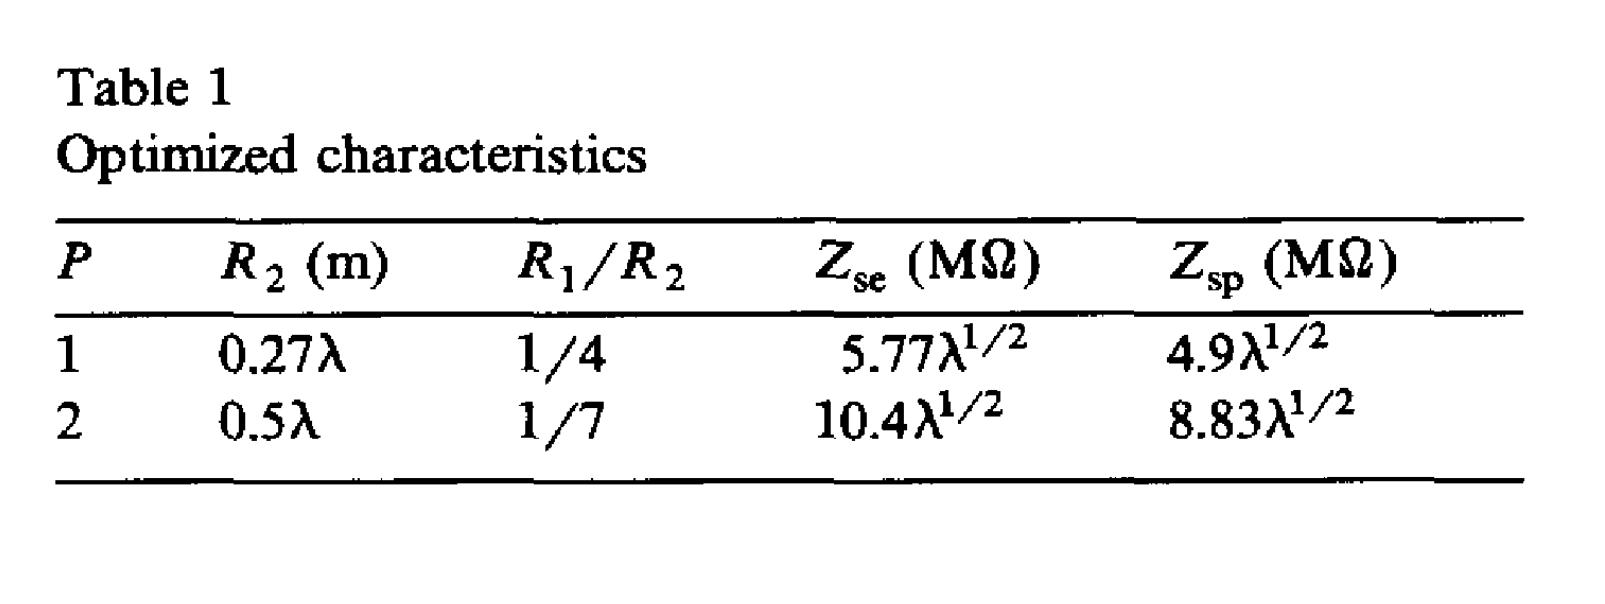
\includegraphics[width=.9\textwidth]{../../../figures/pottier_table1.png}
    \caption{Optimized characteristics of a rhodotron cavity \cite{rhodo_pottier}.}
    \label{fig:pottier_table1}
\end{figure}
Here, $p$ is the integer multiplier in the equation ($l=p\lambda$) mentioned above, $R_1$ is the radius of the inner cylinder, $R_2$ is the radius of the outer cylinder, 
$Z_{se}$ is effective shunt empedance, $Z_{sp}$ is practical shunt empedance which was taken to be $0.85 Z_{se}$. Typically, phase lag $\phi$ is taken as $15^\circ$ \cite{rhodo_pottier}. 

Considering $Z_{sp} \propto \lambda^{1/2}$, \,\,\, $\Delta E \propto \lambda^{1/4}$, \,\,\,   $V \propto \lambda^3$, where $V$ is the volume of the cavity, implementing the $p=1$ design in \fromfig{pottier_table1} is much more space efficient.
\begin{figure}[H]
    \centering
    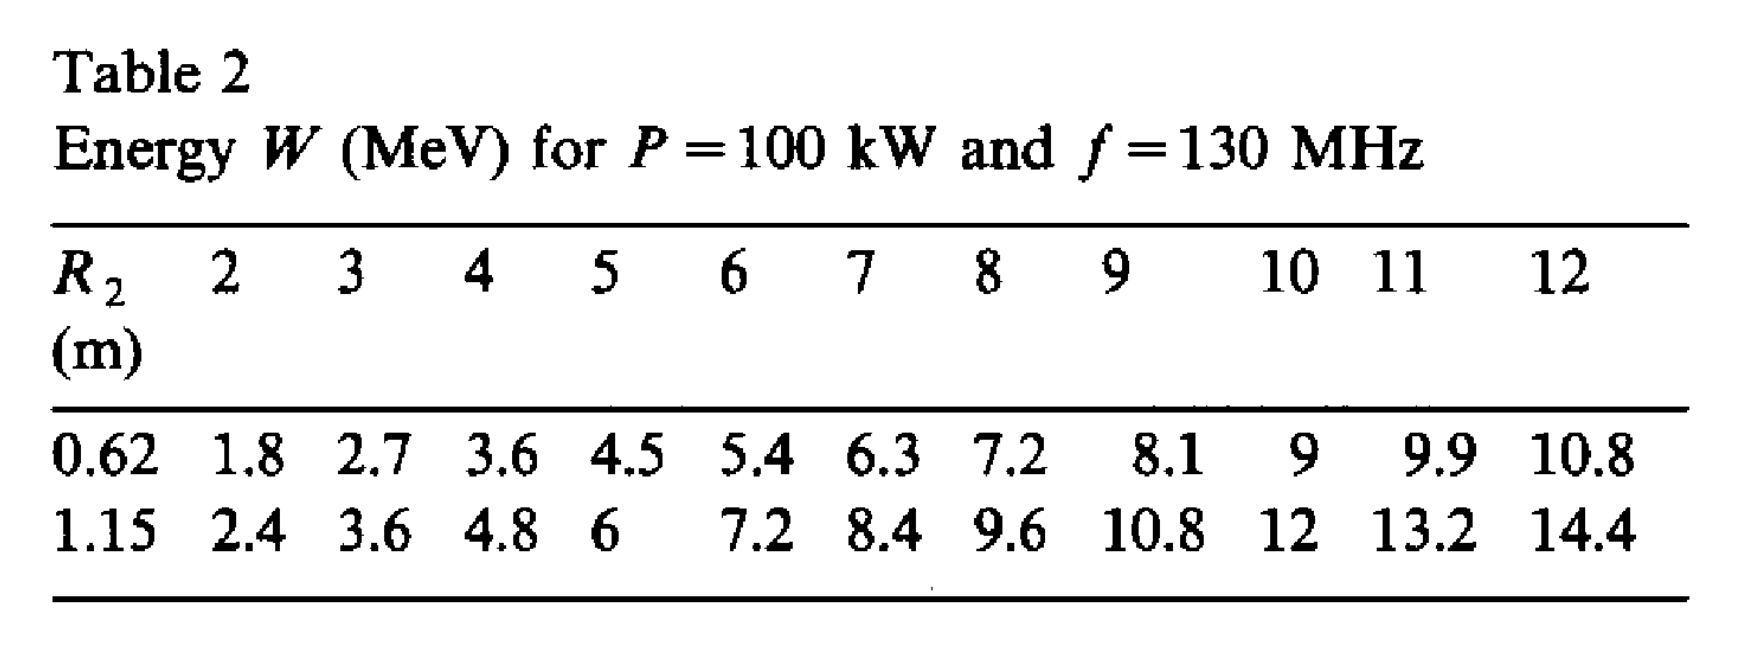
\includegraphics[width=.9\textwidth]{../../../figures/pottier_table2.png}
    \caption{Energy of a synchronous electron after each pass for both $p=1$ and $p=2$ \cite{rhodo_pottier}.}
    \label{fig:pottier_table2}
\end{figure}
Total energy gain after $n$ passes, $\Delta E_n$, can then be found by \fromeq{W_gain_each_pass_pottier}, taking $\phi = 15^\circ$, $p=1$, i.e $R_2 = 0.27 \lambda$, $P$ in \textit{W}, $\lambda$ in \textit{m} as
\vspace{-10pt}\begin{equation}
    \label{eq:W_total_gain_pottier}
    \Delta E_n \approx 2.14 \lambda^{1/4} P^{1/2} n \quad keV .
\vspace{-10pt}\end{equation}


\begin{figure}[H]
    \centering
    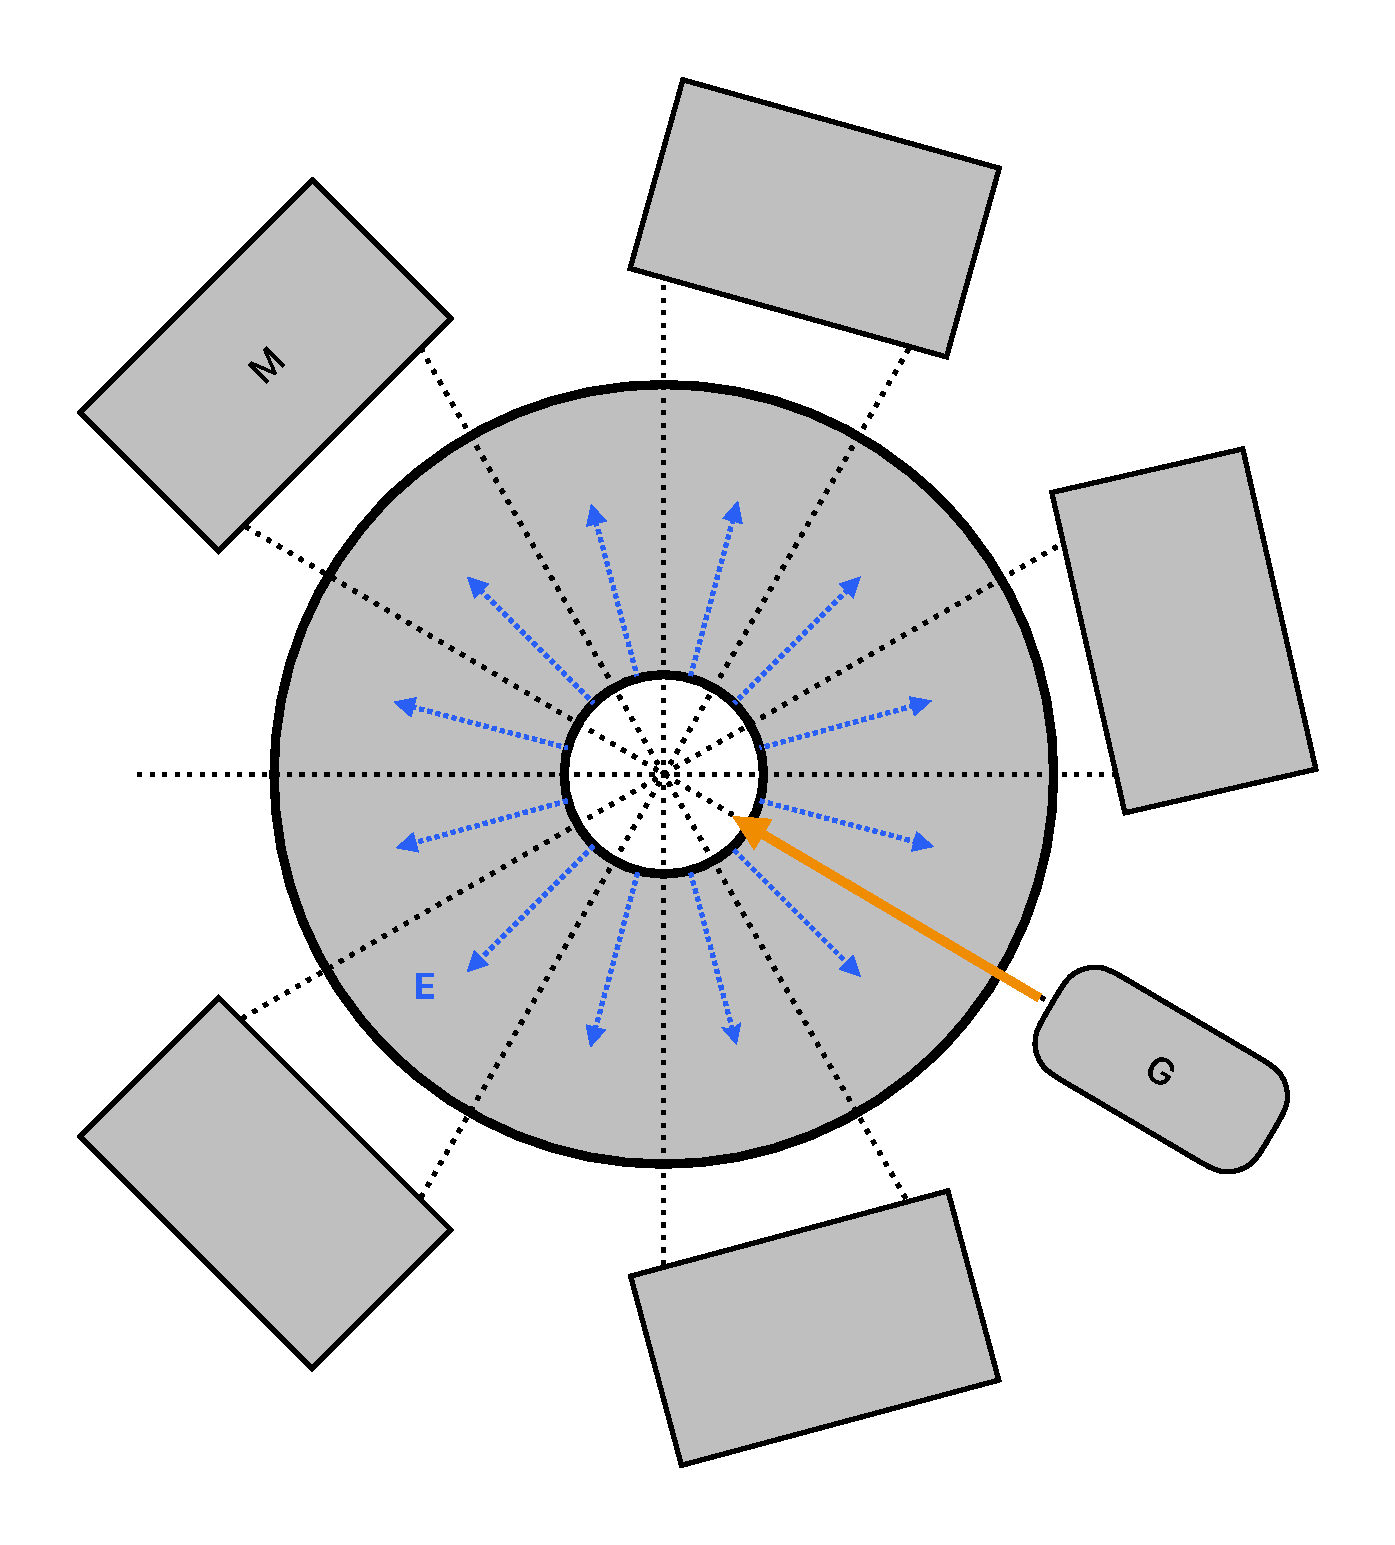
\includegraphics[width=\textwidth]{../../../figures/illustrations/rhod1.pdf}
    \caption{$[0, \frac{T}{4}]$ time frame of a rhodotron.}
    \label{fig:rhod_cycle_1}
\end{figure}
\begin{figure}[H]
    \centering
    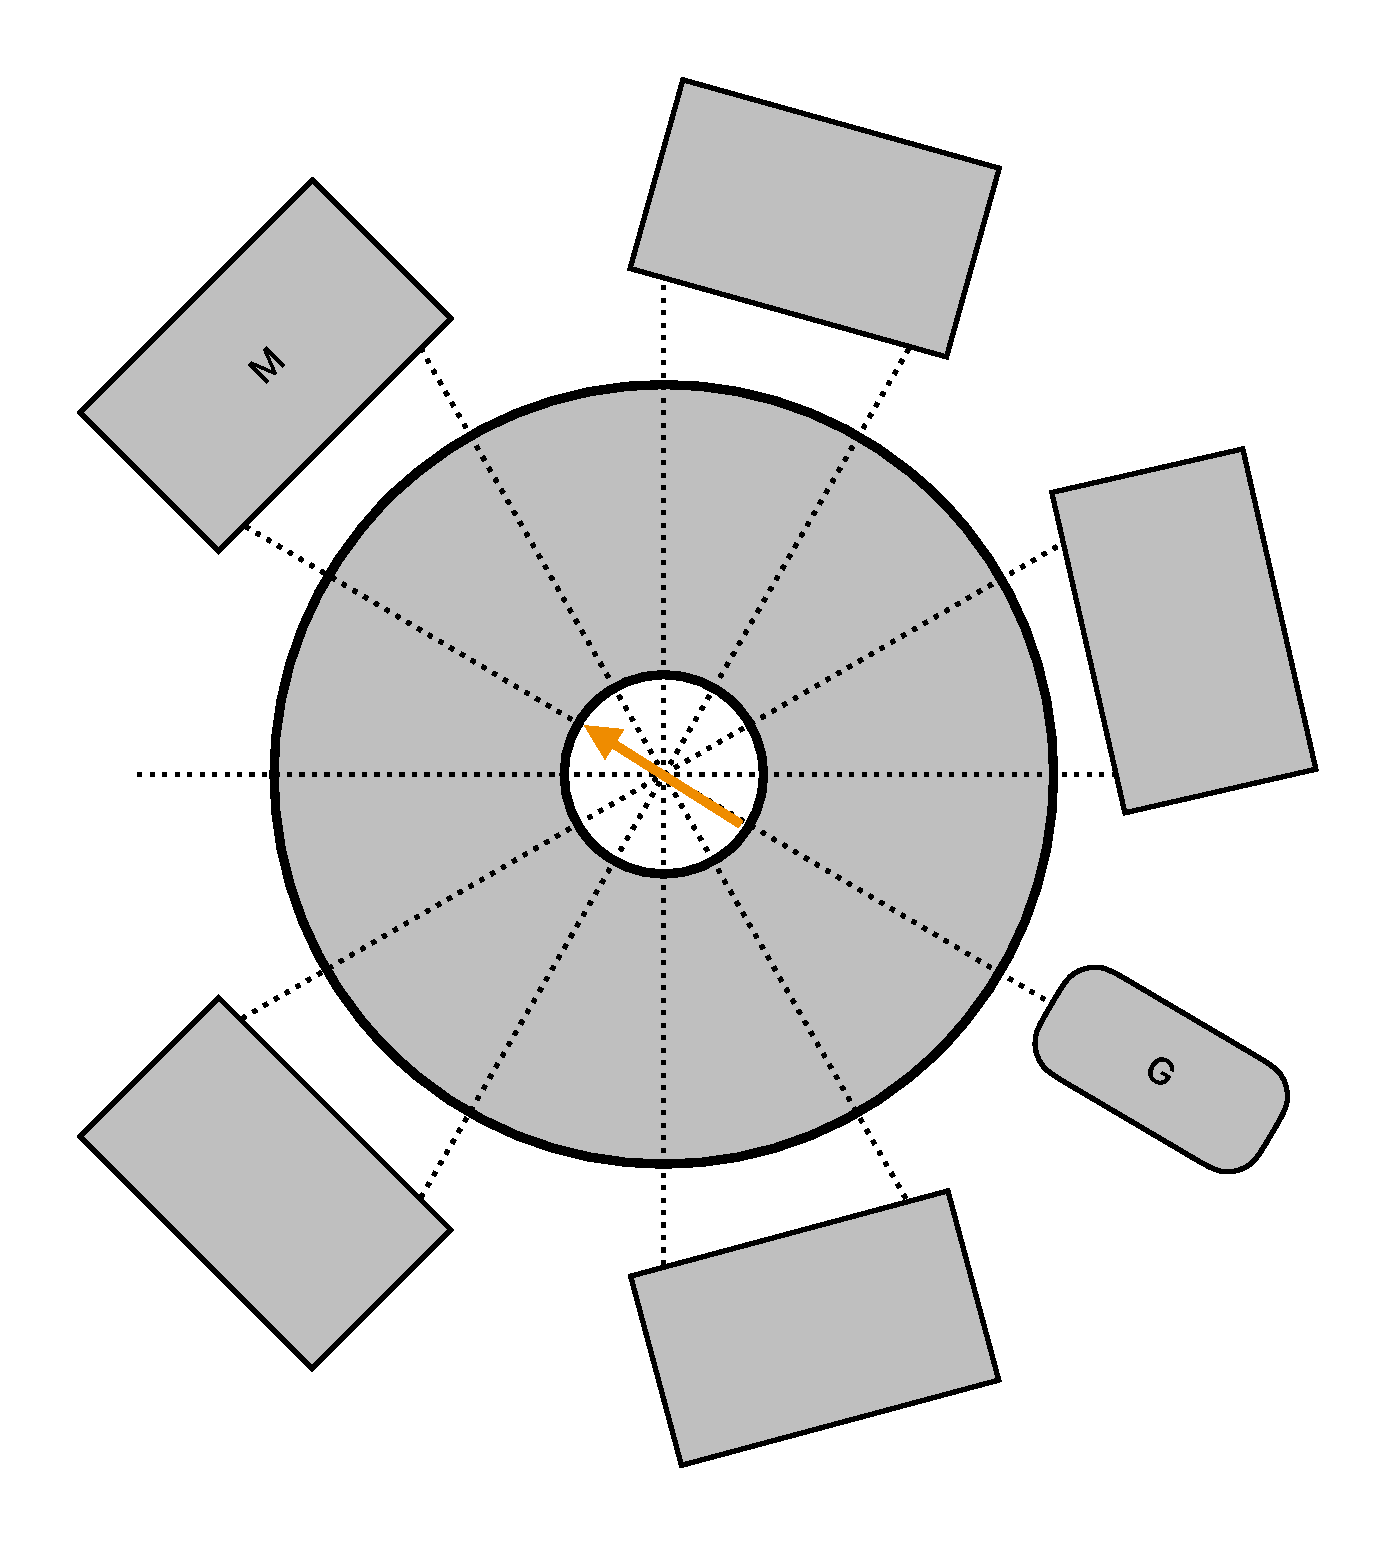
\includegraphics[width=\textwidth]{../../../figures/illustrations/rhod2.pdf}
    \caption{$[\frac{T}{4}, \frac{T}{2}]$ time frame of a rhodotron.}
    \label{fig:rhod_cycle_2}
\end{figure}
\begin{figure}[H]
    \centering
    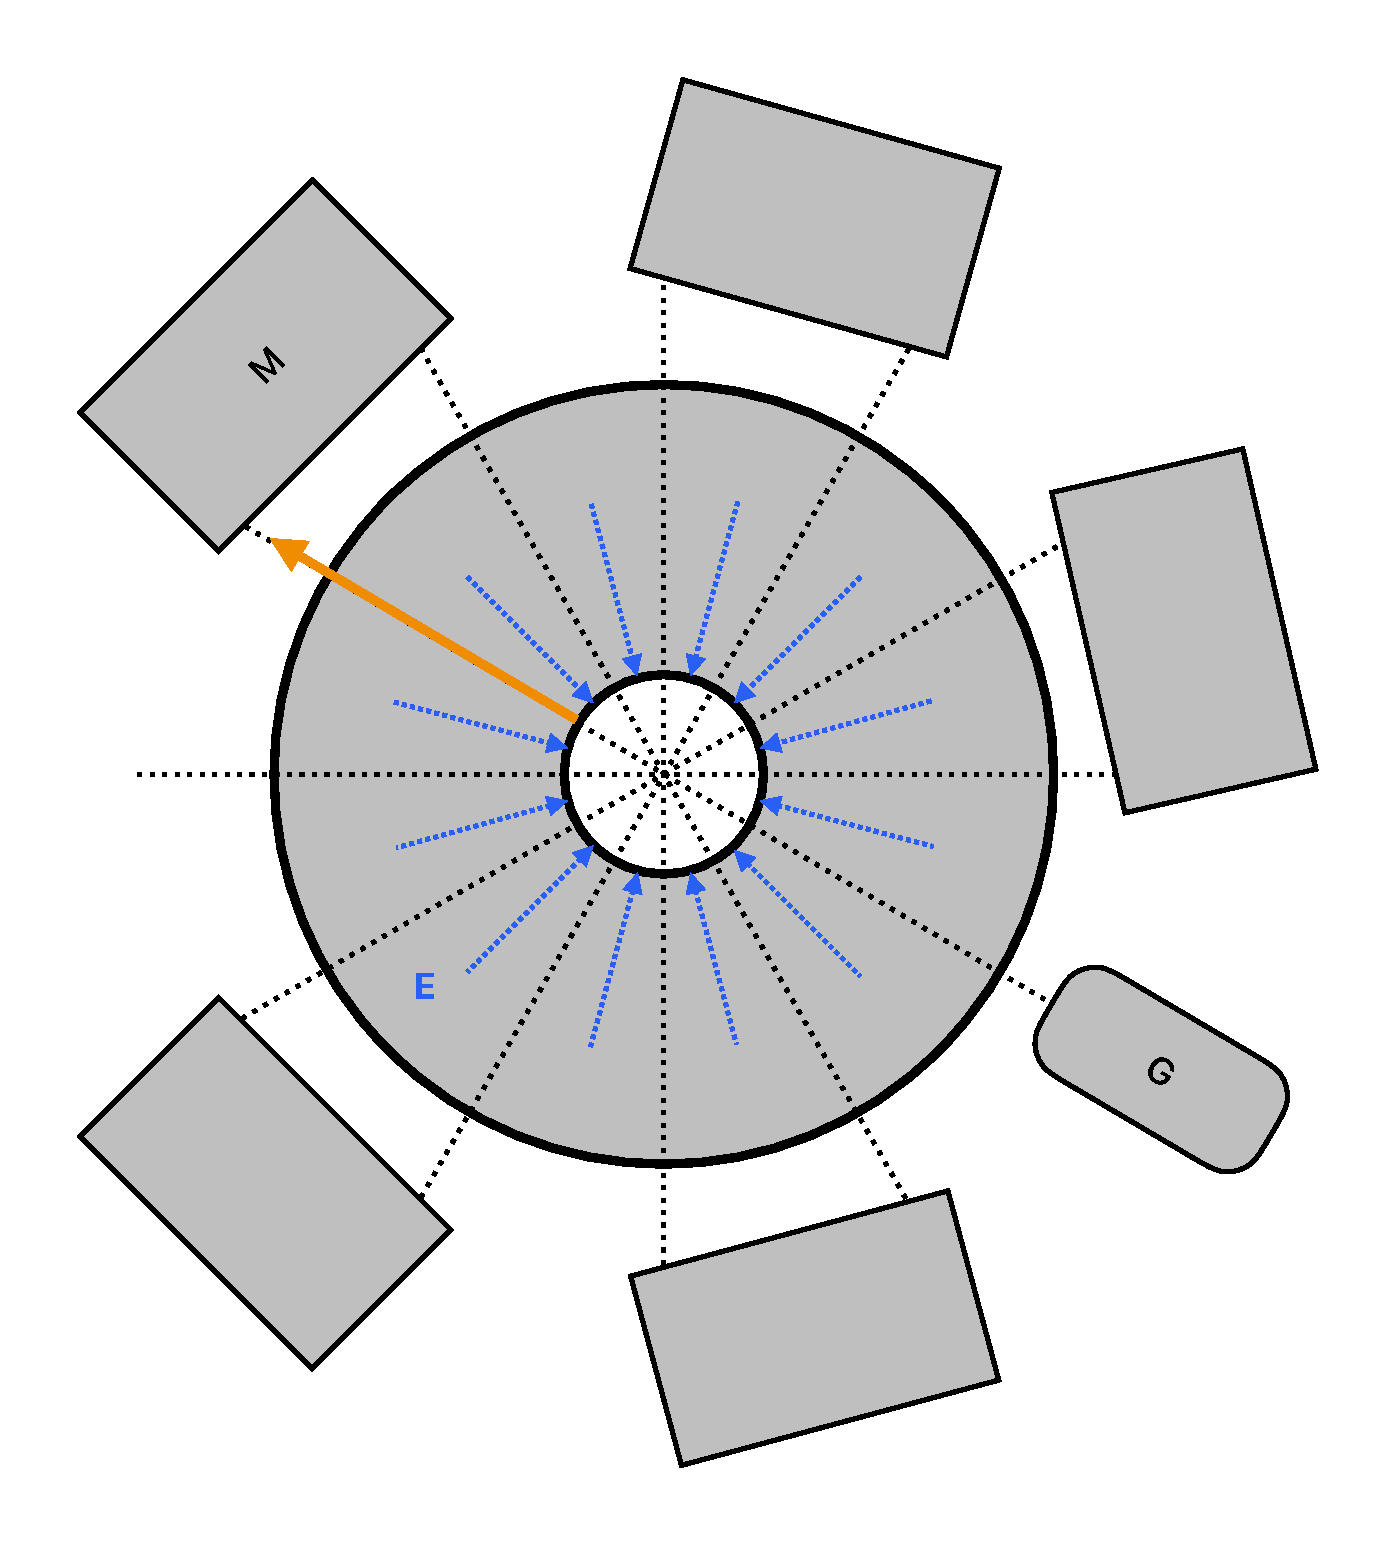
\includegraphics[width=\textwidth]{../../../figures/illustrations/rhod3.pdf}
    \caption{$[\frac{T}{2}, \frac{3T}{4}]$ time frame of a rhodotron.}
    \label{fig:rhod_cycle_3}
\end{figure}
\begin{figure}[H]
    \centering
    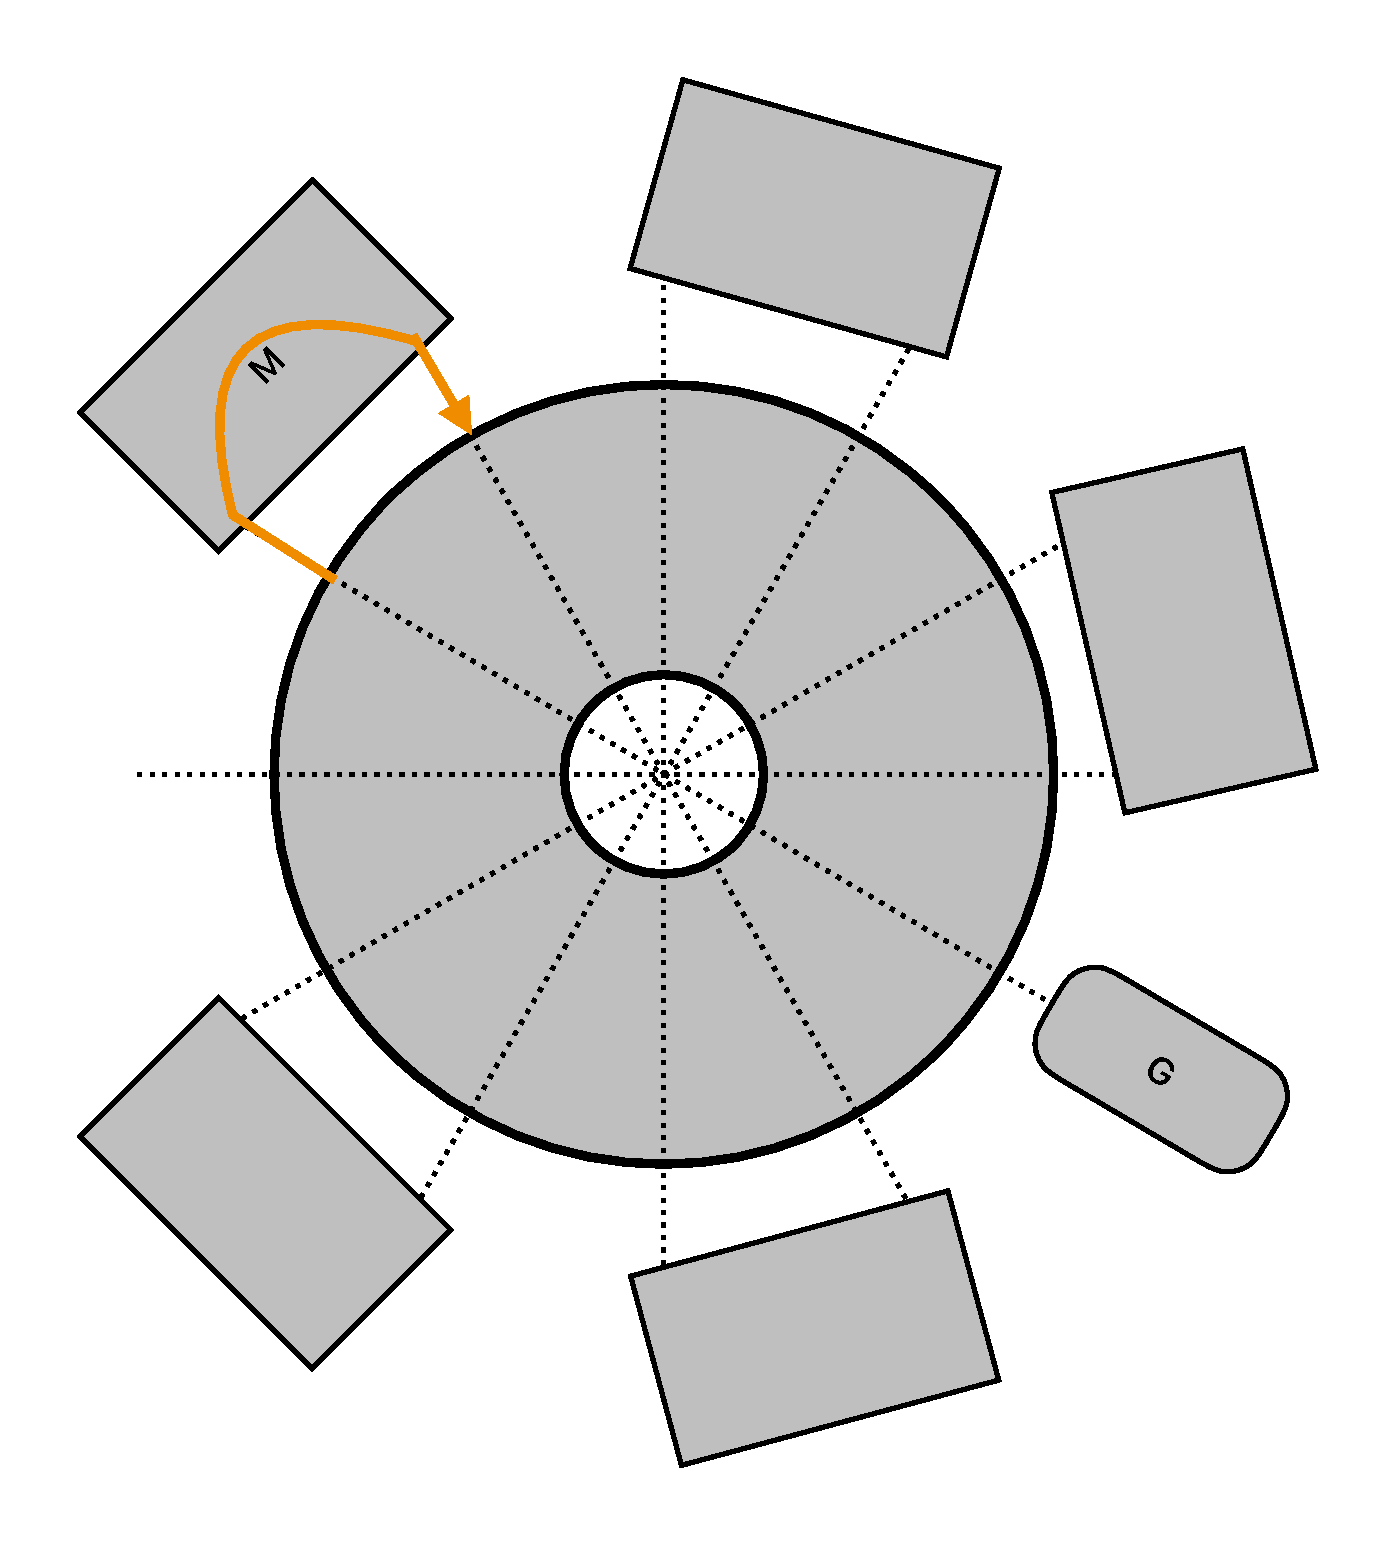
\includegraphics[width=\textwidth]{../../../figures/illustrations/rhod4.pdf}
    \caption{$[\frac{3T}{4}, T]$ time frame of a rhodotron.}
    \label{fig:rhod_cycle_4}
\end{figure}



%%%%%%

\begin{thebibliography}{9}
    \bibitem{rhodo_pottier}
    Jacques Pottier,
    \emph{A new type of rf electron accelerator: The rhodotron},
    Nuclear Instruments and Methods in Physics Research Section B: Beam Interactions with Materials and Atoms,
    Volumes 40–41, Part 2,
    1989,
    Pages 943-945,


    \bibitem{rhodo_prototype}
    J.M. Bassaler, J.M. Capdevila, O. Gal, F. Lainé, A. Nguyen, J.P. Nicolaï, K. Umiastowski,
    \emph{Rhodotron: an accelerator for industrial irradiation},
    Nuclear Instruments and Methods in Physics Research Section B: Beam Interactions with Materials and Atoms,
    Volume 68, Issues 1–4,
    1992,
    Pages 92-95,A:

    \bibitem{rhodos}
    Y. Jongen. (2001). \emph{Manufacturing of Electron Accelerators}. Ion Beam Applications s.a. (IBA) Chemin du Cyclotron 3, B-1348 Louvain-la-Neuve, Belgium.
\end{thebibliography}

\end{document}